% !TEX program = xelatex
% Rencontre Elaia -- mardi 6 octobre 2026
% Participants : Anne-Sophie Carrese (Managing Partner, Elaia), Arturo Ancira García (Associate, Elaia),
%                Louis Hauseux, Alban Hauseux.
% Demande d'Arturo Ancira García : présenter la genèse du projet, la technologie et les applications
%                                  à Anne-Sophie Carrese, partner des fonds deep tech d'Elaia.
% Contenu : transposition du Board meeting #1 (Boards/Board_meeting_1_2026-10-02), avec trois slides en plus :
%           « Genèse du projet » (sources : CV de Louis, dossier de candidature ISS, manuscrit de thèse),
%           « Exemple 4 : arbres urbains (Greehill) » (repris de la présentation au comité ISS du 28 juillet 2026) et
%           « Exemple 5 : rétroconception » (source : W. Gao et G. Li, Deep Learning for 3D Point Clouds, p. 277),
%           puis une slide d'appui pour les vidéos HGP face à HDBSCAN (dépôt E-HGP, dossier Zoltan/, copiées dans videos/).
%           Slide « Au-delà du LiDAR » du Board meeting #1 retirée ; « Du benchmark à la licence logicielle » et
%           « Trois voies d'accès au marché » fusionnées en « Deux voies d'accès au marché », placée avant les exemples.
%           « Exemple 2 : conduite autonome (Valeo AI) », d'après la slide ALPINE de la soutenance.
%           En fin de deck, quatre slides sur le modèle de fondation guidé par la hiérarchie HGP : analogie
%           GPT/SAM, nuage artefact du capteur et figures reprises de la soutenance (dépôt Manuscrit-de-th-se,
%           Soutenance/soutenance), projet décrit dans le dépôt E-HGP, dossier Zoltan/ (en conception).
% Liens LinkedIn : Elaia, ceux de la fiche équipe de chaque participant sur elaia.com ; Alban, son profil
%                  (IMT Atlantique, HSBC, Société Générale) ; Louis, l'URL qu'il a fournie.
%                  Josiane Zerubia et Konstantin Avrachenkov : leur page personnelle Inria.
%                  Gyula Fekete (Greehill) : l'URL fournie par Louis ; Benjamin Berta (Greehill) : celle de la
%                  présentation au comité ISS du 28 juillet 2026.
% Logo Elaia : imgs/Elaia-logo.svg, logo officiel du site elaia.com (icône et wordmark, couleur
%              « green-dark » #143334 du site), rendu en imgs/Elaia-logo.png.
% Thème : thème Inria du Board meeting #1 (dossier theme/ copié à l'identique).
% Compilation : make (XeLaTeX, comme le Board meeting #1).
\documentclass[A4,svgnames,10pt,aspectratio=169,usepdftitle=false]{beamer}

\usepackage[utf8]{inputenc}
\usepackage[english,french]{babel}
\usepackage{graphicx}

\title[Percolia]{\huge \textbf{PERCOLIA}}
\subtitle{\large Structuration automatique de données}
\date[6 octobre 2026]{Mardi 6 octobre 2026}
\author[L. et A. \textsc{Hauseux}]{%
   \href{https://www.linkedin.com/in/louis-hauseux-b80804434}{Louis \textsc{Hauseux}} et \href{https://www.linkedin.com/in/alban-hauseux-9577b6118/}{Alban \textsc{Hauseux}} \\[4pt]
   \footnotesize Rencontre avec \href{https://www.linkedin.com/in/anne-sophie-carrese-566990a6/}{Anne-Sophie \textsc{Carrese}} et \href{https://www.linkedin.com/in/ancirarturo/}{Arturo \textsc{Ancira García}} (Elaia)%
}
\institute{Inria Startup Studio}

% XeTeX ne fournit pas la primitive \draftmode (pdfTeX/LuaTeX), testée par le fond de page du thème
\ifdefined\draftmode\else\chardef\draftmode=0 \fi

\usetheme{inria}

\usetikzlibrary{arrows.meta, positioning, calc, decorations.pathreplacing}
% Boîte du schéma Milla : \bx[style]{nom}{x}{y}{largeur}{hauteur}{couleur}{texte}
\newcommand{\bx}[7][mbx]{\node[#1, fill=#7, minimum width=#5*0.9cm, minimum height=#6*0.76cm, text width=#5*0.9cm-2pt, execute at begin node={\hyphenpenalty=10000\exhyphenpenalty=10000}] (#2) at (#3,#4)}

% Logos de la page de titre : Inria Startup Studio à droite du bloc-marque RF-Inria, Elaia sur la marge droite
\newlength{\isslogowidth}
\newlength{\elaialogowidth}

\hypersetup{
   allcolors   = rouge_inria,
   pdfauthor   = {Louis Hauseux et Alban Hauseux},
   pdftitle    = {PERCOLIA - Rencontre Elaia},
   pdfsubject  = {Présentation de Percolia à Elaia (Anne-Sophie Carrese, Arturo Ancira García) - 6 octobre 2026},
   pdfkeywords = {Percolia, clustering, LiDAR, Inria, HGP-Clusterer, Elaia, deep tech}
}

\begin{document}

% Slide 1 : Page de titre
\begin{frame}
    \titlepage
    \setlength{\isslogowidth}{0.2\textwidth}%
    \begin{textblock*}{\isslogowidth}(\hmargin+\titlelogowidth+3.5mm,\vmargin-\titlelogovoffset)
        
\includegraphics[width=\isslogowidth]{imgs/Inria-StartupStudio-logo.png}
    \end{textblock*}
    % Logo Elaia (342 x 94) centré verticalement sur le logo Inria Startup Studio (480 x 202)
    \setlength{\elaialogowidth}{0.17\textwidth}%
    \begin{textblock*}{\elaialogowidth}[1,0.5](\paperwidth-\hmargin,\vmargin-\titlelogovoffset+\isslogowidth*101/480)
        \href{https://elaia.com/}{
\includegraphics[width=\elaialogowidth]{imgs/Elaia-logo.png}}
    \end{textblock*}
\end{frame}

% Slide 2 : Équipe fondatrice
\begin{frame}{Équipe fondatrice}
    \begin{columns}[T]
        \begin{column}{0.5\textwidth}
            \textbf{\bleu \href{https://www.linkedin.com/in/louis-hauseux-b80804434}{Louis Hauseux}}
            \begin{itemize}
                \item Doctorat en informatique à Inria Sophia Antipolis
                \item Normalien, double master de mathématiques
                \item Concepteur de HGP-Clusterer
                \item Médaille d'excellence de l'Université Côte d'Azur, 2\textsuperscript{e} prix ACM SIGMETRICS, finaliste du prix Pierre \textsc{Laffitte}
            \end{itemize}
        \end{column}

        \begin{column}{0.46\textwidth}
            \textbf{\bleu \href{https://www.linkedin.com/in/alban-hauseux-9577b6118/}{Alban Hauseux}}
            \begin{itemize}
                \item Ingénieur IMT Atlantique, master d'ingénierie financière à Paris-Dauphine
                \item Finance quantitative, audit et contrôle de modèles
                \item Industrialisation, intégration client et développement commercial
            \end{itemize}
        \end{column}
    \end{columns}

    \vspace{0.3cm}
    \textbf{\bleu Conseil scientifique et réseau}
    \begin{itemize}
        \item \href{https://www-sop.inria.fr/members/Josiane.Zerubia/index.html}{Josiane \textsc{Zerubia}}, directrice de recherche Inria, équipe \textsc{Ayana}
    \end{itemize}
\end{frame}

% Slide 3 : Genèse du projet (frise chronologique)
% Sources : CV de Louis (stage de M2 2016-2017 à Inria Paris sur les complexes simpliciaux ; ingénieur de
% recherche Inria févr.-sept. 2023 ; thèse oct. 2023-sept. 2026 ; projet Percolia 2025-2026 ; publications
% « socle de Percolia »), dossier de candidature ISS (« l'origine remonte à un stage de Master 2 fait à l'Inria
% de Paris » ; contacts Greehill et Exwayz ; collaboration avec le projet ISS de Marie Aspro), jury du manuscrit
% de thèse (direction K. Avrachenkov, co-encadrement J. Zerubia).
\begin{frame}{Genèse du projet}
    \centering
    \begin{tikzpicture}[x=0.99\textwidth, y=1cm,
        jalon/.style={circle, fill=inria-rouge, inner sep=0pt, minimum size=2.4mm},
        annee/.style={anchor=south, yshift=2.5mm, font=\small\bfseries, text=inria-2024-bleu-azur},
        etape/.style={anchor=north, yshift=-3.5mm, text width=0.235\textwidth, align=center, inner sep=0pt,
            font=\footnotesize, execute at begin node={\hyphenpenalty=10000\exhyphenpenalty=10000}}]
      \draw[-{Latex[length=2.5mm]}, thick, inria-2024-gris-bleu] (0,0) -- (1,0);
      \foreach \j/\x in {1/0.12, 2/0.37, 3/0.62, 4/0.87} \node[jalon] (j\j) at (\x,0) {};
      \node[annee] at (j1) {2017};
      \node[etape] at (j1) {\textbf{Origine}\\ Stage de master~2 à Inria Paris sur les complexes simpliciaux};
      \node[annee] at (j2) {2023};
      \node[etape] at (j2) {\textbf{Ingénieur de recherche}\\ Inria Sophia Antipolis\\ Graphes géométriques et \emph{clustering}};
      \node[annee] at (j3) {2023--2026};
      \node[etape] at (j3) {\textbf{Thèse}\\ Encadrée par \href{https://www-sop.inria.fr/members/Konstantin.Avratchenkov/me.html}{K.~\textsc{Avrachenkov}} et \href{https://www-sop.inria.fr/members/Josiane.Zerubia/index.html}{J.~\textsc{Zerubia}}\\ Conception de HGP-Clusterer\\ Soutenue le 8~septembre~2026};
      \node[annee, text=inria-2024-orange] at (j4) {2025--2026};
      \node[etape] at (j4) {\textbf{Percolia}\\ Échanges avec Greehill, Exwayz et AI Detech\\ Starthèse, VivaTech, DeepTech Forum\\ Inria Startup Studio depuis octobre~2026};
    \end{tikzpicture}

    \vfill
    \raggedright
    \textbf{\orange Fil conducteur} Des paires de points aux interactions d'ordre supérieur, pour un \emph{clustering} robuste au bruit

    \vspace{0.2cm}
    {\tiny \textcolor{inria-2024-gris-bleu}{Publications EUSIPCO 2024, \emph{Complex Networks} 2025, \emph{ACM SIGMETRICS PER} 2025, \emph{Applied Network Science} 2026}\par}
\end{frame}

% Slide 4 : La limite des méthodes actuelles de clustering
\begin{frame}{La limite des méthodes actuelles de \emph{clustering}}
    \textbf{\bleu Les standards DBSCAN et HDBSCAN}
    \begin{itemize}
        \item Repèrent les zones denses puis relient les points deux à deux
        \item Rapides, disponibles partout et très utilisés
    \end{itemize}

    \vspace{0.25cm}
    \textbf{\bleu Le problème dans les scènes LiDAR réelles}
    \begin{itemize}
        \item Le bruit crée des ponts entre objets voisins
        \item Ces objets fusionnent alors (effet de chaînage)
    \end{itemize}

    \vspace{0.25cm}
    \textbf{\orange Conséquence} Mauvaise segmentation, anomalies mal isolées, corrections manuelles
\end{frame}

% Slide 5 : La rupture technique de Percolia
\begin{frame}{La rupture technique de Percolia}
    \textbf{\bleu HGP-Clusterer généralise le \emph{Single-Linkage}}
    \begin{itemize}
        \item Des connexions évaluées entre groupes de points, et non plus entre deux points
        \item Une hiérarchie de groupes à toutes les échelles, qui retarde les fusions dues au bruit
    \end{itemize}

    \vspace{0.2cm}
    \begin{columns}[T]
        \begin{column}{0.48\textwidth}
            \textbf{\bleu Propriétés du moteur}
            \begin{itemize}
                \item Sans entraînement ni annotation
                \item Compatible avec un changement de capteur ou de domaine
                \item Conçu pour de grands nuages de points
            \end{itemize}
        \end{column}

        \begin{column}{0.48\textwidth}
            \textbf{\bleu Spécificité industrielle}
            \begin{itemize}
                \item Volumes, dimensions ou modèles 3D guident le choix des groupes
                \item S'insère dans un \emph{pipeline} existant
            \end{itemize}
        \end{column}
    \end{columns}

    \vfill
    {\tiny \textcolor{inria-2024-gris-bleu}{L.~\textsc{Hauseux}, K.~\textsc{Avrachenkov}, J.~\textsc{Zerubia}, «~\href{https://doi.org/10.1007/s41109-025-00756-1}{\foreignlanguage{english}{Generalization of Single-Linkage with Higher-Order Interactions}}~», \emph{Applied Network Science}, 2026}\par}
\end{frame}

% Slide 6 : Le LiDAR comme premier marché
\begin{frame}{Le LiDAR comme premier marché}
    \begin{columns}[T]
        \begin{column}{0.48\textwidth}
            \textbf{\bleu Point d'entrée commercial}
            \begin{itemize}
                \item Jumeaux numériques, suivi d'actifs, inspection industrielle
                \item Clients déjà équipés de scanners et d'un \emph{pipeline} 3D
                \item Scènes bruitées aux objets imbriqués
            \end{itemize}
        \end{column}
        \begin{column}{0.48\textwidth}
            \textbf{\bleu Valeur mesurable}
            \begin{itemize}
                \item Moins de fusions erronées
                \item Moins de corrections manuelles
                \item Une étape plus facile à automatiser
            \end{itemize}
        \end{column}
    \end{columns}
\end{frame}

% Slide 7 : Deux voies d'accès au marché
% D'après « Du benchmark à la licence logicielle » et « Trois voies d'accès au marché » du Board meeting #1,
% regroupées en deux axes : roadmap produit (benchmark, intégration, licence ou API, puis logiciel des
% constructeurs LiDAR) et verticale complète.
\begin{frame}{Deux voies d'accès au marché}
    \textbf{\bleu \emph{Roadmap} produit}

    \vspace{0.2cm}
    \centering
    \begin{tikzpicture}[x=0.99\textwidth, y=1cm,
        jalon/.style={circle, fill=inria-rouge, inner sep=0pt, minimum size=2.4mm},
        etape/.style={anchor=south, yshift=2.5mm, text width=0.235\textwidth, align=center, inner sep=0pt,
            font=\small\bfseries, text=inria-2024-bleu-azur, execute at begin node={\hyphenpenalty=10000\exhyphenpenalty=10000},
            execute at end node={\strut}},
        detail/.style={anchor=north, yshift=-3.5mm, text width=0.235\textwidth, align=center, inner sep=0pt,
            font=\footnotesize, execute at begin node={\hyphenpenalty=10000\exhyphenpenalty=10000}},
        accolade/.style={decorate, decoration={brace, mirror, amplitude=4pt}, gray},
        noms/.style={below=6pt, align=center, font=\small, text=black}]
      \draw[-{Latex[length=2.5mm]}, thick, inria-2024-gris-bleu] (0,0) -- (1,0);
      \foreach \j/\x in {1/0.12, 2/0.37, 3/0.62, 4/0.87} \node[jalon] (j\j) at (\x,0) {};
      \node[etape] at (j1) {\emph{Benchmark} ou pilote};
      \node[detail] at (j1) {Sur quelques scans du client};
      \node[etape] at (j2) {Intégration};
      \node[detail] at (j2) {Dans le \emph{pipeline} du client};
      \node[etape] at (j3) {Licence ou API};
      \node[detail] at (j3) {Revenu logiciel récurrent};
      \node[etape] at (j4) {Constructeurs LiDAR};
      \node[detail] at (j4) {Notre moteur dans le logiciel de leurs scanners};
      \draw[accolade] (0.005,-1.25) -- (0.735,-1.25)
        node[midway, noms] {\href{https://www.greehill.com/}{Greehill}, \href{https://www.linkedin.com/company/ai-detech}{AI Detech}, \href{https://www.milla-group.com/}{Milla}, \href{https://www.hydroquebec.com/}{Hydro-Québec}};
      \draw[accolade] (0.755,-1.25) -- (0.985,-1.25)
        node[midway, noms] {\href{https://www.yellowscan.com/}{YellowScan}, \href{https://www.artec3d.com/}{Artec 3D}};
    \end{tikzpicture}

    \vfill
    \raggedright
    \textbf{\bleu Verticale complète}
    \begin{itemize}
        \item Le service complet, de la donnée brute au résultat
    \end{itemize}
\end{frame}

% Slide 8 : Exemple 1 : chantiers navals (AI Detech)
\begin{frame}{Exemple 1 : chantiers navals (AI Detech)}
    \begin{columns}[T,onlytextwidth]
        \begin{column}{0.53\textwidth}
            \textbf{\bleu Projet ISS avec Naval Group}
            \begin{itemize}
                \item \textbf{Objectif} Détecter les anomalies de chantier
                \item \textbf{Données} Modèle 3D attendu face aux captations LiDAR (synthétiques par confidentialité)
                \item \textbf{Percolia} Isoler ce qui n'est pas dans le modèle (casques, tuteurs, bâches)
            \end{itemize}
            \textbf{\bleu Le verrou}
            \begin{itemize}
                \item Un \emph{clustering} fin, guidé par le modèle 3D
            \end{itemize}
        \end{column}

        \begin{column}{0.43\textwidth}
            \centering
            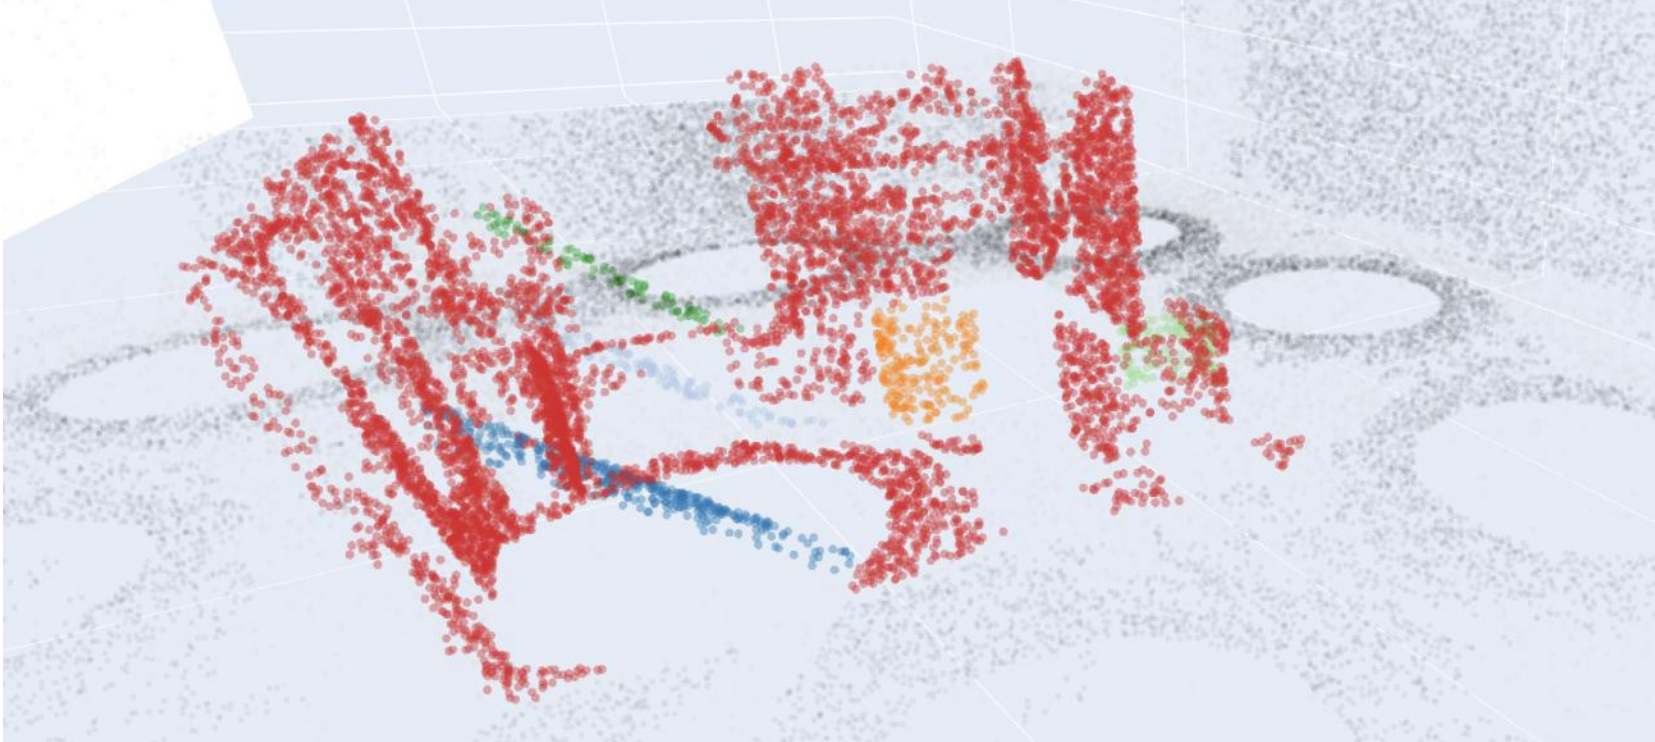
\includegraphics[width=\textwidth]{imgs/Resultat_MarieBenchmark.png}\\
            \tiny \textcolor{inria-2024-gris-bleu}{Modèle 3D en rouge, anomalies en orange, vert et bleu\\ © Marie \textsc{Aspro} et Naval Group}
        \end{column}
    \end{columns}

    \vfill
    \textbf{\orange Interlocutrice} \href{https://www.linkedin.com/in/m-aspro/}{Marie \textsc{Aspro}}, depuis la Fête des start-ups de l'ISS en novembre 2025
\end{frame}

% Slide 9 : Exemple 2 : conduite autonome (Valeo AI)
% D'après la slide de soutenance « Panoptique 3D : l'état de l'art est un clustering » (image imgs/Alpine.png).
% Références : Sautier et al. 2025 (arXiv:2503.13203), Oh et al. 2025 (arXiv:2512.18991).
% Lien avec la thèse (annexe « Colloques & formations ») : séminaire donné chez Valeo AI le 24 novembre 2025,
% « Méthodes de clustering avec graphes. Ou "Comment hacker (H)DBSCAN ?" » ; contact avec Renaud Marlet,
% Principal Scientist à Valeo.ai et coauteur d'ALPINE.
\begin{frame}{Exemple 2 : conduite autonome (Valeo AI)}
    \small
    \begin{columns}[T,onlytextwidth]
        \begin{column}{0.56\textwidth}
            \textbf{\bleu ALPINE, l'état de l'art sur LiDAR extérieur}
            \begin{itemize}
                \item \textbf{Panoptique} La classe de chaque point et son instance
                \item \textbf{Avant} Des instances apprises, au prix d'annotations coûteuses
                \item \textbf{ALPINE} La sémantique puis un \emph{clustering} classique sans apprentissage, repris en 4D par Geo-4D
            \end{itemize}
            \textbf{\bleu Le verrou}
            \begin{itemize}
                \item Un graphe à rayon fixe, qui peut fusionner des objets proches
            \end{itemize}
        \end{column}

        \begin{column}{0.40\textwidth}
            \centering
            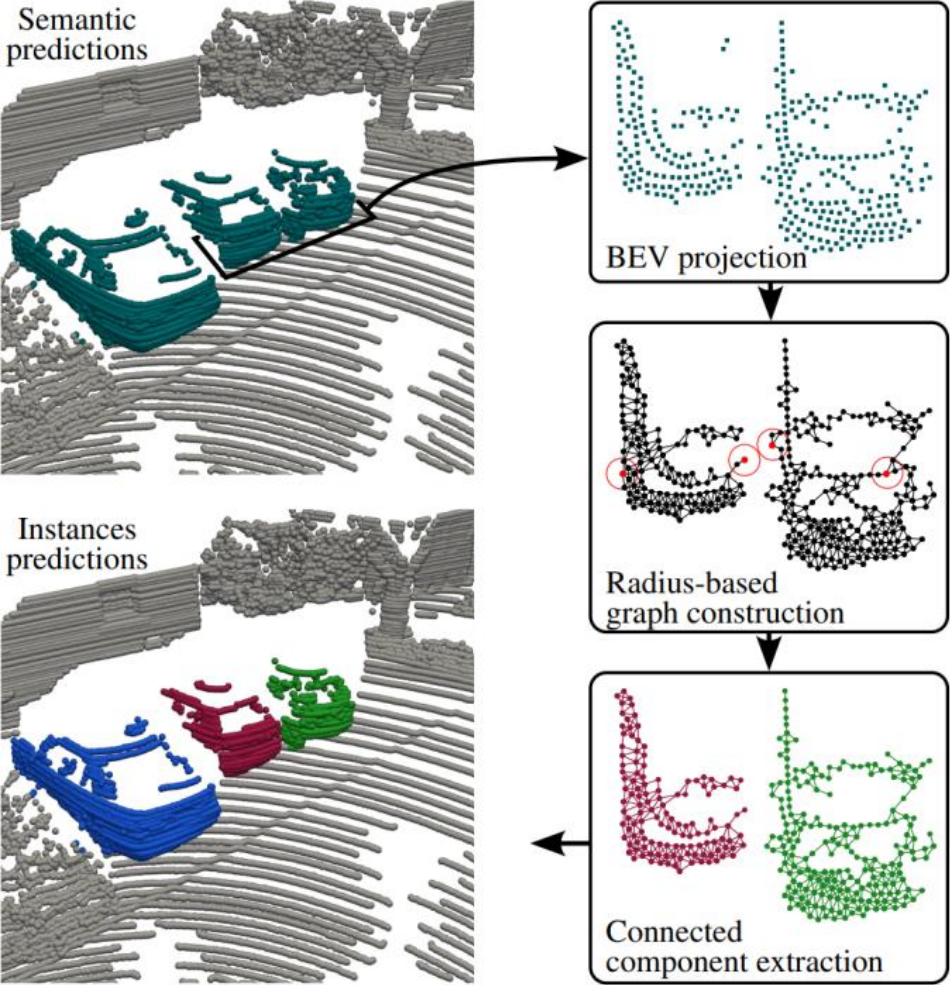
\includegraphics[height=0.5\textheight]{imgs/Alpine.png}\\
            \tiny \textcolor{inria-2024-gris-bleu}{Chaîne d'ALPINE, de la sémantique aux instances}
        \end{column}
    \end{columns}

    \vfill
    \textbf{\orange Interlocuteur} \href{https://imagine.enpc.fr/~marletr/}{Renaud \textsc{Marlet}}, coauteur d'ALPINE, depuis le séminaire «~Comment \emph{hacker} (H)DBSCAN~?~» donné chez Valeo AI en novembre 2025

    \vspace{0.1cm}
    {\tiny \textcolor{inria-2024-gris-bleu}{C.~\textsc{Sautier} \emph{et al.}, «~\href{https://arxiv.org/abs/2503.13203}{\foreignlanguage{english}{Is clustering enough for LiDAR instance segmentation? A state-of-the-art training-free baseline}}~» (ALPINE), 2025\\
    G.~\textsc{Oh} \emph{et al.}, «~\href{https://arxiv.org/abs/2512.18991}{\foreignlanguage{english}{Training-free global geometric association for 4D LiDAR panoptic segmentation}}~» (Geo-4D), 2025}\par}
\end{frame}

% Slide 10 : Exemple 3 : navette autonome (Milla), détection d'obstacles
% Schéma reproduit d'après la diapositive «~Détection obstacles~» présentée par Milla
% aux Scientific Days (25 septembre 2026, Pôle Alpha, Sophia Antipolis).
\definecolor{milla-radar}{HTML}{8BAA4A}
\definecolor{milla-lidar}{HTML}{8FD14F}
\definecolor{milla-camera}{HTML}{D7B9A8}
\definecolor{milla-violet}{HTML}{9F4DBE}
\definecolor{milla-gris}{HTML}{8DA8BD}
\begin{frame}{Exemple 3 : navette autonome (Milla)}
    \centering
    \begin{tikzpicture}[x=0.9cm, y=-0.76cm, font=\scriptsize, >={Latex[length=1.3mm]},
        mbx/.style={draw=gray!70, fill=white, align=center, inner sep=1pt, text=black!75},
        mcap/.style={draw=gray!60, align=center, inner sep=1pt, text=white},
        ln/.style={draw=gray!70, ->, thin}]
      % Capteurs
      \bx[mcap]{radar}{2.84}{2.79}{2.9}{0.48}{milla-radar}{Radar};
      \bx[mcap]{lidar}{7.45}{2.85}{2.85}{0.48}{milla-lidar}{Lidar};
      \bx[mcap]{camera}{13.57}{2.84}{2.88}{0.46}{milla-camera}{Camera};
      % Chaîne radar
      \bx{radardet}{2.81}{4.17}{2.9}{1.28}{white}{Radar Object Detection};
      % Chaîne lidar
      \bx[mcap]{prefilt}{7.45}{3.63}{2.85}{0.42}{milla-violet}{Lidar pre-filtering};
      \bx{cluster}{6.73}{4.47}{1.43}{0.9}{white}{\tiny 3D Object Detection Cluster};
      \bx{ia}{8.24}{4.47}{1.43}{0.9}{white}{\tiny 3D Object Detection IA};
      \bx[mcap]{pretrack}{7.42}{5.85}{3.05}{0.62}{milla-gris}{Pretracker\_Fusion};
      \bx[mcap]{map}{7.42}{6.74}{3.05}{0.6}{milla-gris}{Map filter};
      \bx[mcap]{mot}{7.42}{7.63}{3.05}{0.62}{milla-gris}{Multi object tracker};
      \bx[mcap]{pred}{7.42}{8.55}{3.05}{0.6}{milla-gris}{Prediction map filtering};
      \bx[mcap]{occ}{7.42}{9.43}{3.05}{0.6}{milla-gris}{Occupancy Grid Map};
      % Chaîne caméra
      \bx{person}{12.33}{3.77}{2.3}{0.98}{white}{2D Person Detection (Yolo)};
      \bx{traffic}{14.75}{3.80}{2.16}{0.98}{white}{2D Traffic Light Detection (Yolo)};
      \bx{frustum}{12.57}{5.06}{2.3}{0.98}{white}{frustrum};
      % Légende
      \bx[mcap]{sensor}{14.71}{9.43}{2.9}{0.42}{milla-violet}{Sensor dependant};
      % Flèches
      \draw[ln] (radar) -- (radardet);
      \draw[ln] (radardet.south) -- (radardet.south |- mot.west) -- node[above, font=\tiny\itshape, text=black!70, pos=0.6] {Object velocity} (mot.west);
      \draw[ln] (lidar) -- (prefilt);
      \draw[ln] (cluster.north |- prefilt.south) -- (cluster);
      \draw[ln] (ia.north |- prefilt.south) -- (ia);
      \draw[ln] (cluster) -- (cluster |- pretrack.north);
      \draw[ln] (ia) -- (ia |- pretrack.north);
      \draw[ln] (pretrack) -- (map);
      \draw[ln] (map) -- (mot);
      \draw[ln] (mot) -- (pred);
      \draw[ln] (pred) -- (occ);
      \draw[ln] (prefilt.east) -- (10.15,3.63) -- (10.15,5.06) -- (frustum.west);
      \draw[ln] (camera.south) -- (person.north);
      \draw[ln] (camera.south) -- (traffic.north);
      \draw[ln] (person) -- (frustum);
      \draw[ln] (frustum.south) -- (frustum.south |- mot.east) -- (mot.east);
      \draw[ln] ([yshift=-1.5pt]mot.east) -- ++(0.3,0) |- (pretrack.east);
      % Partie concernée par Percolia
      \draw[inria-rouge, very thick, rounded corners=2pt] ([shift={(-2pt,2pt)}]cluster.north west) rectangle ([shift={(2pt,-2pt)}]cluster.south east);
      \node[text=inria-rouge, font=\scriptsize\bfseries, anchor=east, align=right] at ([xshift=-5pt]cluster.west) {\emph{Clustering}\\Percolia};
    \end{tikzpicture}

    \vspace{0.1cm}
    {\tiny \textcolor{inria-2024-gris-bleu}{D'après la présentation de \href{https://www.milla-group.com/}{Milla} aux Scientific Days (Sophia Antipolis, septembre 2026)\quad © Milla}\par}
\end{frame}

% Slide 11 : Exemple 4 : arbres urbains (Greehill)
% Repris de l'exemple 2 de Presentation_Inria_Startup_Studio_2026-07-28 (comité ISS du 28 juillet 2026).
% Étapes et images d'après la présentation de Greehill (documents/GreeHill.pdf, p. 25, « How do we extract
% insights from the point cloud? ») : Semantic Segmentation et Wood-leaf separation, Instance Segmentation,
% 3D representation. imgs/Greehill_Tree_Instances.png et imgs/Greehill_Tree_3D.png sont des copies de
% Greehill_Wood_Leaf_After.png et de Greehill_Instance_Segmentation.png (présentation de juillet), renommées
% d'après leur contenu.
\begin{frame}{Exemple 4 : arbres urbains (\href{https://www.greehill.com/}{Greehill})}
    \begin{columns}[T,onlytextwidth]
        \begin{column}{0.52\textwidth}
            \textbf{\bleu Inventaire intelligent des arbres}
            \begin{itemize}
                \item Jumeaux numériques par LiDAR mobile
                \item Santé, chutes de branches, obstacles proches
            \end{itemize}
        \end{column}
        \begin{column}{0.44\textwidth}
            \textbf{\bleu Le verrou}
            \begin{itemize}
                \item Le feuillage se mêle aux lignes électriques, aux panneaux et aux façades
            \end{itemize}
        \end{column}
    \end{columns}

    \vfill
    \centering
    \begin{tikzpicture}[>={Latex[length=1.6mm]}, image/.style={inner sep=0pt},
        legende/.style={anchor=north, yshift=-1.5mm, align=center, font=\scriptsize}]
      \node[image] (semantique) {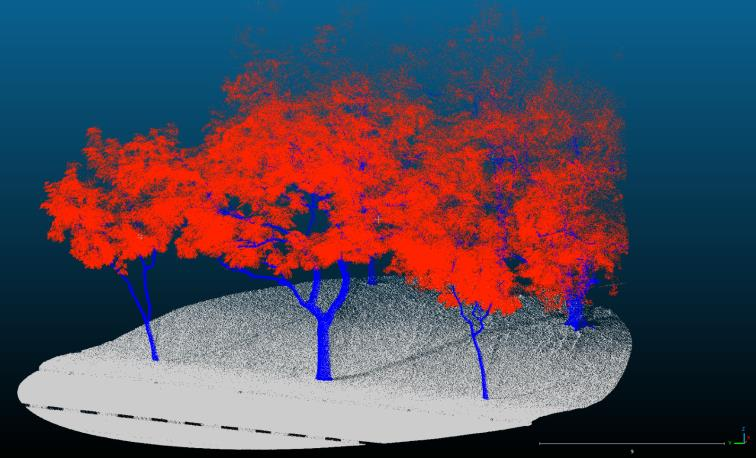
\includegraphics[height=1.6cm]{imgs/Greehill_Semantic_Segmentation.png}};
      \node[image, right=1.2cm of semantique] (instances) {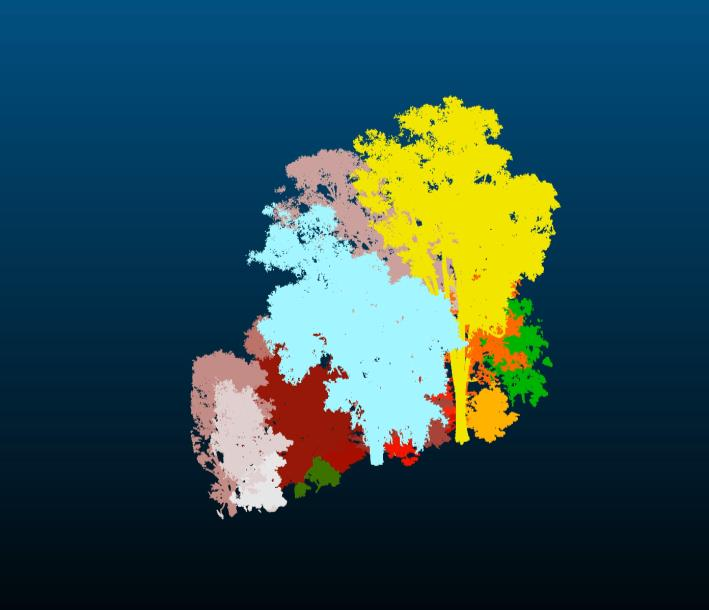
\includegraphics[height=1.6cm]{imgs/Greehill_Tree_Instances.png}};
      \node[image, right=1.2cm of instances] (arbre) {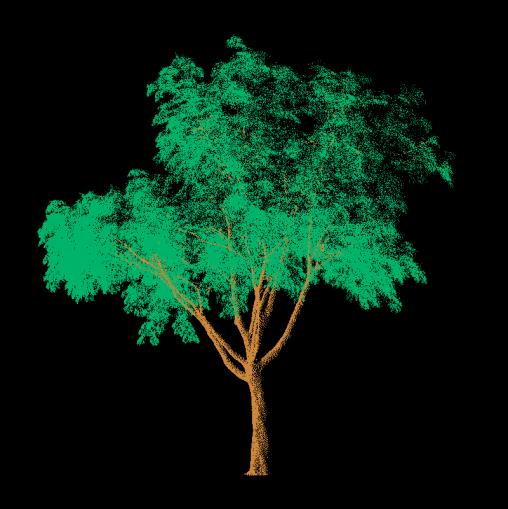
\includegraphics[height=1.6cm]{imgs/Greehill_Tree_3D.png}};
      \draw[->, thick] (semantique) -- (instances);
      \draw[->, thick] (instances) -- (arbre);
      \node[legende] at (semantique.south) {Segmentation sémantique\\ (sol, bois, feuilles)};
      \node[legende] at (instances.south) {Séparation\\ des arbres};
      \node[legende] at (arbre.south) {Modèle 3D\\ de chaque arbre};
      % Partie concernée par Percolia
      \draw[inria-rouge, very thick, rounded corners=2pt] ([shift={(-3pt,3pt)}]instances.north west) rectangle ([shift={(3pt,-3pt)}]instances.south east);
      \node[text=inria-rouge, font=\small\bfseries, anchor=south] at ([yshift=5pt]instances.north) {\emph{Clustering} Percolia};
    \end{tikzpicture}

    \vfill
    \raggedright
    \textbf{\orange Interlocuteur} \href{https://www.linkedin.com/in/benjamin-berta/}{Benjamin \textsc{Berta}}, échanges en 2025 sur leur brique DBSCAN

    \vspace{0.1cm}
    {\tiny \textcolor{inria-2024-gris-bleu}{Images extraites d'une présentation de \href{https://www.linkedin.com/in/gyula-szabolcs-fekete-6a029112/}{Gyula \textsc{Fekete}} (Greehill), rencontré à l'école d'été SSRM 2024 à Veszprém}\par}
\end{frame}

% Slide 12 : Exemple 5 : rétroconception (reverse engineering)
% Schéma adapté (intitulés traduits) de la Fig. 10.1 « Pipeline of reverse engineering » de W. Gao et G. Li,
% Deep Learning for 3D Point Clouds, Springer Nature Singapore, 2025, chap. 10 « Typical Engineering
% Applications of 3D Point Clouds », p. 277 : Data Collection, Data Processing, Model Refactoring, Rapid Production.
\definecolor{gaoli-peche}{HTML}{F8CBAD}
\begin{frame}{Exemple 5 : rétroconception}
    La rétroconception (\emph{reverse engineering}) recrée le modèle numérique d'un objet existant à partir de sa numérisation 3D

    \vfill
    \centering
    \begin{tikzpicture}[x=0.99\textwidth, y=1cm, >={Latex[length=1.6mm]},
        etape/.style={fill=gaoli-peche, rounded corners=3pt, minimum width=0.2\textwidth, minimum height=1.3cm,
            text width=0.17\textwidth, align=center, font=\normalsize, text=black}]
      \node[etape] (scan) at (0.12,0) {Numérisation 3D};
      \node[etape] (traitement) at (0.37,0) {Traitement des données};
      \node[etape] (modele) at (0.62,0) {Modèle 3D};
      \node[etape] (fabrication) at (0.87,0) {Fabrication};
      \draw[->, thick] (scan) -- (traitement);
      \draw[->, thick] (traitement) -- (modele);
      \draw[->, thick] (modele) -- (fabrication);
      % Cadre pointillé de la figure d'origine
      \draw[gray!60, dashed, rounded corners=4pt] ([shift={(-6pt,6pt)}]scan.north west) rectangle ([shift={(6pt,-6pt)}]fabrication.south east);
      % Partie concernée par Percolia
      \draw[inria-rouge, very thick, rounded corners=2pt] ([shift={(-3pt,3pt)}]traitement.north west) rectangle ([shift={(3pt,-3pt)}]traitement.south east);
      \node[text=inria-rouge, font=\small\bfseries, anchor=south] at ([yshift=9pt]traitement.north) {Percolia};
    \end{tikzpicture}

    \vfill
    {\tiny \textcolor{inria-2024-gris-bleu}{Schéma adapté de la fig.~10.1 de W.~\textsc{Gao} et G.~\textsc{Li}, \href{https://doi.org/10.1007/978-981-97-9570-3}{\emph{Deep Learning for 3D Point Clouds}}, Springer, 2025, p.~277}\par}
\end{frame}

% Slide 13 : HGP-Clusterer face à HDBSCAN (slide d'appui pour lancer les vidéos)
% Vidéos du dépôt E-HGP (dossier Zoltan/), copiées dans videos/ ; chaque scène ouvre sa vidéo.
% Ce que montrent les vidéos (même k pour les deux hiérarchies, r = rayon des boules d'ordre k, et pour
% HDBSCAN distance d'atteignabilité mutuelle / 2) :
%   08/002852, k = 5, deux vélos garés côte à côte près d'un bâtiment : HDBSCAN fusionne A avec le bâtiment
%     (r = 7,1 cm) puis réunit A et B (7,6 cm), B jamais retrouvé ; HGP retrouve A (IoU 0,77) et B (0,88)
%   08/001170, k = 5, deux vélos imbriqués : HDBSCAN réunit A et B à 8,7 cm (B jamais retrouvé) ;
%     HGP A 0,93 et B 0,72
%   06/000800, k = 10, un piéton et deux vélos près d'un bâtiment : HDBSCAN réunit B et C à 11,4 cm
%     (jamais retrouvés) ; HGP A 0,99, B 0,74, C 0,74
%   00/002140, k = 10, un piéton tout près d'un vélo : HDBSCAN réunit A et B à 8,3 cm (B jamais retrouvé) ;
%     HGP A 0,94 et B 0,87
\begin{frame}{HGP-Clusterer face à HDBSCAN}
    \small
    \textbf{\bleu Le principe}
    \begin{itemize}
        \item \textbf{Hiérarchie} Le rayon $r$ grandit, les groupes se forment puis fusionnent
        \item \textbf{IoU} Intersection sur union d'un groupe et d'un objet réel, de 0 à 1
        \item \textbf{Objet retrouvé} Un groupe de la hiérarchie dépasse un IoU de 0,5
        \item \textbf{Lecture} HGP à gauche, HDBSCAN à droite, même $k$
    \end{itemize}

    \vspace{0.2cm}
    \textbf{\bleu Des endroits difficiles}
    \begin{columns}[T,onlytextwidth]
        \begin{column}{0.5\textwidth}
            \begin{itemize}
                \item \href{run:videos/08_002852_deux_velos_6_51_sans_sol_k5_clair.mp4}{Deux vélos près d'un bâtiment} {\scriptsize\textcolor{inria-2024-gris-bleu}{08/002852}}
                \item \href{run:videos/08_001170_deux_velos_43_57_sans_sol_k5_clair.mp4}{Deux vélos imbriqués} {\scriptsize\textcolor{inria-2024-gris-bleu}{08/001170}}
            \end{itemize}
        \end{column}
        \begin{column}{0.48\textwidth}
            \begin{itemize}
                \item \href{run:videos/06_000800_pieton_deux_velos_2_8_12_sans_sol_k10_clair.mp4}{Un piéton et deux vélos} {\scriptsize\textcolor{inria-2024-gris-bleu}{06/000800}}
                \item \href{run:videos/00_002140_pieton_velo_1_6_instances_k10_clair.mp4}{Un piéton tout près d'un vélo} {\scriptsize\textcolor{inria-2024-gris-bleu}{00/002140}}
            \end{itemize}
        \end{column}
    \end{columns}

    \vfill
    \textbf{\orange À retenir} HDBSCAN réunit trop tôt les objets voisins, HGP les retrouve tous

    Pour la supériorité théorique de HGP, voir \href{https://doi.org/10.1007/s41109-025-00756-1}{\emph{Applied Network Science}, 2026}

    \vspace{0.1cm}
    {\tiny \textcolor{inria-2024-gris-bleu}{Données SemanticKITTI, HDBSCAN de scikit-learn}\par}
\end{frame}

% Slide 14 : Vers un modèle de fondation pour la 3D
% Analogie de la soutenance de thèse du 8 septembre 2026 (« Les modèles de fondation : le texte, et
% désormais l'image » et « Vers un modèle de fondation pour la 3D ? »), figure figs/alphabet_fondation.tex.
\begin{frame}{Vers un modèle de fondation pour la 3D ?}
    \begin{center}
        \resizebox{0.86\textwidth}{!}{% Figure reprise de la soutenance de thèse (dépôt Manuscrit-de-th-se, Soutenance/soutenance/figs/alphabet_fondation.tex),
% références remplacées par l'éditeur et l'année, note du bas simplifiée.
                \begin{tikzpicture}[xscale=1.0, yscale=1.0]
                    \useasboundingbox (-0.35, -2.05) rectangle (13.35, 3.35);

                    \tikzset{jeton/.style={draw=inria-2024-bleu-canard, line width=0.7pt, rounded corners=1.5pt,
                                           fill=inria-2024-bleu-canard!12, inner sep=2pt, font=\scriptsize,
                                           minimum height=4.2mm}}
                    \tikzset{modele/.style={draw=gris_fonce_inria, line width=1.0pt, rounded corners=3pt,
                                            fill=gray!8, inner sep=4pt, font=\small\bfseries, minimum width=1.55cm,
                                            minimum height=6.5mm}}
                    \tikzset{modeleouvert/.style={modele, draw=inria-rouge, fill=inria-rouge!6, text=inria-rouge}}
                    \tikzset{fl/.style={-{Latex[length=2.2mm]}, line width=0.9pt, color=gray!55}}
                    \tikzset{dom/.style={font=\small, anchor=east, text=gris_fonce_inria}}

                    % ---------------- ligne 1 : le langage ----------------
                    \node[dom] at (1.35, 2.75) {\textbf{langage}};
                    \node[jeton, anchor=west] (t1) at (1.75, 2.75) {Les};
                    \node[jeton, anchor=west] (t2) at ($(t1.east)+(0.09,0)$) {graph};
                    \node[jeton, anchor=west] (t3) at ($(t2.east)+(0.09,0)$) {es};
                    \node[jeton, anchor=west] (t4) at ($(t3.east)+(0.09,0)$) {sont};
                    \node[jeton, anchor=west] (t5) at ($(t4.east)+(0.09,0)$) {partout};
                    \node[font=\scriptsize, text=inria-2024-bleu-canard, anchor=west] at ($(t5.east)+(0.25,0)$) {sous-mots};
                    \node[modele, anchor=west] (m1) at (9.85, 2.75) {GPT};
                    \node[anchor=west, font=\scriptsize, text=gris_fonce_inria] at ($(m1.east)+(0.14,0)$) {OpenAI, 2020};
                    \draw[fl] (8.55, 2.75) -- (m1.west);

                    % ---------------- ligne 2 : l'image ----------------
                    \node[dom] at (1.35, 1.45) {\textbf{image}};
                    \begin{scope}[shift={(1.80,0.80)}]
                        \foreach \i in {0,...,4} {
                            \foreach \j in {0,...,2} {
                                \draw[inria-2024-bleu-canard, line width=0.6pt, fill=inria-2024-bleu-canard!12]
                                    (\i*0.44, \j*0.44) rectangle ++(0.40,0.40);
                            }
                        }
                    \end{scope}
                    \node[font=\scriptsize, text=inria-2024-bleu-canard, anchor=west] at (4.25, 1.45) {imagettes};
                    \node[modele, anchor=west] (m2) at (9.85, 1.45) {SAM};
                    \node[anchor=west, font=\scriptsize, text=gris_fonce_inria] at ($(m2.east)+(0.14,0)$) {Meta, 2023};
                    \draw[fl] (8.55, 1.45) -- (m2.west);

                    % ---------------- ligne 3 : la 3D ----------------
                    \node[dom] at (1.35, 0.05) {\textbf{monde 3D}};
                    \begin{scope}[shift={(1.80,-0.55)}]
                        \foreach \x/\y in {0.05/0.10, 0.22/0.52, 0.38/0.86, 0.55/0.30, 0.74/0.68, 0.92/1.02,
                                           1.10/0.16, 1.28/0.60, 1.44/0.94, 1.62/0.38, 1.80/0.76, 1.98/0.22,
                                           0.15/0.72, 0.66/0.98, 1.20/0.92, 1.72/1.04, 0.44/0.44, 0.98/0.48} {
                            \fill[inria-2024-bleu-canard] (\x, \y) circle (1.6pt);
                        }
                    \end{scope}
                    \node[font=\scriptsize, text=inria-2024-bleu-canard, anchor=west] at (4.25, 0.05) {points du capteur};
                    \node[modeleouvert, anchor=west] (m3) at (9.85, 0.05) {?};
                    \node[font=\scriptsize, text=gris_fonce_inria, anchor=north, align=center] at (10.62, -0.30)
                        {Sonata, Concerto,\\Utonia\ldots};
                    \draw[fl, color=inria-rouge!55, densely dashed] (8.55, 0.05) -- (m3.west);

                    % ---------------- séparateur ----------------
                    \draw[gray!35, line width=0.6pt] (0.55, 0.62) -- (11.9, 0.62);

                    % ---------------- accolade et question ----------------
                    \node[font=\scriptsize, align=center, text=inria-rouge, anchor=north] at (5.4, -1.05)
                        {en 3D, l'unité de calcul reste le \textbf{point du capteur}\\
                         ou la case d'une grille};
                \end{tikzpicture}
}
    \end{center}

    \vfill
    \begin{itemize}
        \item Entraîné une fois sur des données massives sans annotation, puis réutilisé partout
        \item Le texte a GPT, l'image a SAM, la 3D cherche encore le sien
    \end{itemize}
\end{frame}

% Slide 15 : Le nuage est un artefact du capteur
% Reprise de la soutenance de thèse (« La raison de fond : le nuage est un artefact du capteur »),
% figure figs/verrou_portee.tex.
\begin{frame}{Le nuage est un artefact du capteur}
    \begin{center}
        \resizebox{0.66\textwidth}{!}{% Figure reprise de la soutenance de thèse (dépôt Manuscrit-de-th-se, Soutenance/soutenance/figs/verrou_portee.tex),
% légende de droite sans deux-points.
                \begin{tikzpicture}[xscale=1.0, yscale=1.0]
                    \useasboundingbox (-0.45, -2.85) rectangle (13.35, 2.25);

                    \tikzset{pt/.style={circle, fill=inria-2024-bleu-canard, inner sep=0pt, minimum size=2.2pt}}
                    \tikzset{surf/.style={inria-rouge, line width=1.6pt, line join=round, line cap=round}}
                    \tikzset{carrosserie/.style={draw=gray!45, line width=0.7pt, fill=gray!8, line join=round}}
                    \tikzset{rayon/.style={gris_fonce_inria, line width=0.35pt, opacity=0.40}}
                    \tikzset{cadre/.style={draw=gray!30, line width=0.9pt, rounded corners=3pt}}

                    \newcommand{\voiture}{%
                        \draw[carrosserie]
                            (0.00,0.00) -- (0.00,0.42) -- (0.48,0.46) -- (0.92,0.98)
                            -- (2.00,0.98) -- (2.42,0.46) -- (3.00,0.42) -- (3.00,0.00) -- cycle;
                        \draw[gray!45, line width=0.7pt] (0.70,0.00) circle (0.20);
                        \draw[gray!45, line width=0.7pt] (2.30,0.00) circle (0.20);
                    }
                    \newcommand{\contour}{(0.00,0.42) (0.48,0.46) (0.92,0.98) (2.00,0.98) (2.42,0.46) (3.00,0.42)}

                    % ================== Panneau gauche : de près ==================
                    \begin{scope}[xshift=0.4cm, yshift=0.35cm]
                        \node[cadre, minimum width=5.0cm, minimum height=2.30cm] at (1.5,0.60) {};
                        \voiture
                        % Nappes de balayage tous les 0.108 : l'une longe le capot et le coffre
                        % (0.44), une autre le toit (0.98) ; chaque retour est à l'intersection
                        % d'une nappe et du contour (pas 0.108 le long d'une nappe).
                        \foreach \y in {0.224, 0.332, 0.440, 0.548, 0.656, 0.764, 0.872, 0.980, 1.088} {\draw[rayon] (-0.55,\y) -- (3.55,\y);}
                        \foreach \p in {(0.020,0.440),(0.128,0.440),(0.236,0.440),(0.344,0.440),(0.452,0.440),(0.555,0.548),(0.646,0.656),(0.738,0.764),(0.829,0.872),(0.980,0.980),(1.088,0.980),(1.196,0.980),(1.304,0.980),(1.412,0.980),(1.520,0.980),(1.628,0.980),(1.736,0.980),(1.844,0.980),(1.952,0.980),(2.087,0.872),(2.174,0.764),(2.261,0.656),(2.348,0.548),(2.450,0.440),(2.558,0.440),(2.666,0.440),(2.774,0.440),(2.882,0.440),(2.990,0.440)} {
                            \node[pt] at \p {};
                        }
                        \node[font=\small, text=gris_fonce_inria, anchor=north] at (1.5,-0.44) {objet \textbf{proche}};
                    \end{scope}

                    % ================== Panneau droit : de loin ==================
                    \begin{scope}[xshift=6.9cm, yshift=0.35cm]
                        \node[cadre, minimum width=5.0cm, minimum height=2.30cm] at (1.5,0.60) {};
                        \voiture
                        % Nappes 2,5 fois plus espacées (0.27) et retours 3 fois plus espacés
                        % le long d'une nappe (0.34) : neuf retours sur trois nappes.
                        \foreach \y in {0.17, 0.44, 0.71, 0.98, 1.25} {\draw[rayon] (-0.55,\y) -- (3.55,\y);}
                        \foreach \p in {(0.080,0.440),(0.420,0.440),(0.692,0.710),(1.100,0.980),(1.440,0.980),(1.780,0.980),(2.218,0.710),(2.580,0.440),(2.920,0.440)} {
                            \node[pt] at \p {};
                        }
                        \node[font=\small, text=gris_fonce_inria, anchor=north] at (1.5,-0.44) {objet \textbf{lointain}};
                    \end{scope}

                    % ================== Flèches ==================
                    \draw[-{Latex[length=2.8mm]}, line width=1.6pt, color=gray!45] (1.90,-0.95) -- (1.90,-1.28);
                    \draw[-{Latex[length=2.8mm]}, line width=1.6pt, color=gray!45] (8.40,-0.95) -- (8.40,-1.28);

                    % ================== Surfaces reconstruites ==================
                    % à gauche : fine ; à droite : grossière, mais même cible
                    \begin{scope}[xshift=0.4cm, yshift=-2.40cm]
                        \draw[gray!45, line width=0.7pt, densely dotted] plot coordinates {\contour};
                        \draw[surf] plot coordinates {\contour};
                    \end{scope}
                    \begin{scope}[xshift=6.9cm, yshift=-2.40cm]
                        \draw[gray!45, line width=0.7pt, densely dotted] plot coordinates {\contour};
                        % La surface interpole les neuf retours observés : ses sommets sont
                        % sur le contour gris, les cordes coupent les angles. Grossière, mais
                        % c'est bien le même objet, c'est tout le propos de la planche.
                        \draw[surf] plot coordinates {(0.080,0.440) (0.420,0.440) (0.692,0.710) (1.100,0.980) (1.440,0.980) (1.780,0.980) (2.218,0.710) (2.580,0.440) (2.920,0.440)};
                    \end{scope}

                    \node[font=\Large\bfseries, text=inria-rouge] at (6.15,-1.86) {$\approx$};

                    \node[font=\scriptsize, text=inria-2024-bleu-canard, anchor=east, align=right] at (12.45,0.95)
                        {le \textbf{nuage}\\dépend du capteur\\et de la portée};
                    \node[font=\scriptsize, text=inria-rouge, anchor=east, align=right] at (12.45,-1.90)
                        {la \textbf{surface} varierait\\beaucoup moins\\selon notre \emph{hypothèse}};
                \end{tikzpicture}
}
    \end{center}

    \vfill
    \begin{itemize}
        \item Densité décroissante avec la portée, nappes de balayage, occultations
        \item Un modèle point par point apprend à la fois la géométrie, le capteur, la densité, l'occultation et la sémantique
    \end{itemize}

    \vfill
    \textbf{\orange Hypothèse} C'est \emph{une} raison centrale de la difficulté
\end{frame}

% Slide 16 : Sémantique et instances, inverser l'ordre
% Dans les exemples (Greehill) comme dans l'état de l'art ALPINE (Sautier et al., Valeo AI, 2025, présenté
% à la soutenance) : sémantique apprise d'abord, puis clustering classe par classe pour les instances.
\begin{frame}{Sémantique et instances : inverser l'ordre}
    Dans nos exemples comme dans l'état de l'art, la sémantique vient d'abord et le \emph{clustering} ensuite

    \vfill
    \centering
    \begin{tikzpicture}[>={Latex[length=1.8mm]},
        etape/.style={draw=gris_fonce_inria, line width=0.8pt, rounded corners=3pt, fill=gray!8,
            minimum width=3cm, text width=2.8cm, minimum height=1.1cm, align=center, font=\small},
        hgp/.style={etape, draw=inria-rouge, fill=inria-rouge!6, line width=1.2pt},
        ligne/.style={font=\small\bfseries, anchor=east}]
      \node[ligne, text=gris_fonce_inria] at (0,0) {Aujourd'hui};
      \node[etape] (p1) at (1.7,0) {Points LiDAR};
      \node[etape] (s1) at (5.4,0) {Sémantique\\ {\scriptsize réseau appris}};
      \node[etape] (i1) at (9.1,0) {Instances\\ {\scriptsize \emph{clustering}}};
      \draw[->, thick] (p1) -- (s1);
      \draw[->, thick] (s1) -- (i1);
      \node[ligne, text=inria-rouge] at (0,-1.7) {Notre piste};
      \node[etape] (p2) at (1.7,-1.7) {Points LiDAR};
      \node[hgp] (h2) at (5.4,-1.7) {Hiérarchie HGP\\ {\scriptsize sans apprentissage}};
      \node[etape] (s2) at (9.1,-1.7) {Sémantique et instances\\ {\scriptsize guidées par la hiérarchie}};
      \draw[->, thick] (p2) -- (h2);
      \draw[->, thick] (h2) -- (s2);
    \end{tikzpicture}

    \vfill
    \raggedright
    \textbf{\orange Hypothèse} Le \emph{clustering} hiérarchique HGP est assez bon pour aider la sémantique
\end{frame}

% Slide 17 : Un modèle de fondation guidé par HGP
% Figure figs/hierarchie_surfaces.tex de la soutenance (« Remplacer les points par une hiérarchie de
% polyèdres ? »). Projet HGP-FM : dépôt E-HGP, dossier Zoltan/, collaboration Inria et université de Szeged
% (Louis Hauseux, Zoltán Kató, Josiane Zerubia), en conception, aucun résultat revendiqué.
\begin{frame}{Un modèle de fondation guidé par HGP}
    \begin{columns}[c,onlytextwidth]
        \begin{column}{0.44\textwidth}
            \centering
            \resizebox{\textwidth}{!}{% Figure reprise telle quelle de la soutenance de thèse (dépôt Manuscrit-de-th-se, Soutenance/soutenance/figs/hierarchie_surfaces.tex).
                    % Hierarchie de K-polyedres proposee comme unite de calcul a la place du point.
                    % Les six pieces des feuilles sont les six secteurs d'un meme polygone maitre
                    % irregulier (decoupe en eventail autour d'un point interieur O). Elles sont
                    % dessinees partout a la meme echelle et dans la meme orientation : le polyedre
                    % d'un noeud interne est donc litteralement le recollement de ceux de ses deux
                    % enfants, soude le long de la face tracee en rouge epais. L'ordonnee est le
                    % rayon physique r ; le point rouge d'un noeud est place en O, au coeur du polyedre.
                    \begin{tikzpicture}[xscale=1.0, yscale=1.0]
                    \useasboundingbox (-1.70, -0.40) rectangle (10.303, 7.541);

                    \tikzset{arbre/.style={gris_fonce_inria!75, line width=0.9pt}}
                    \tikzset{bord/.style={draw=inria-2024-bleu-canard, line width=1.05pt, line join=round}}
                    \tikzset{couture/.style={draw=inria-2024-bleu-canard!70, line width=0.4pt}}
                    \tikzset{soudure/.style={draw=inria-rouge, line width=1.7pt}}

                    % ==== axe des rayons ====
                    \draw[-{Latex[length=2.4mm]}, gris_fonce_inria, line width=0.8pt] (-1.00,-0.25) -- (-1.00,7.271);
                    \node[font=\scriptsize, text=gris_fonce_inria, anchor=south] at (-1.00,7.341) {$r$};
                    \draw[gris_fonce_inria, line width=0.6pt] (-1.00,0.6) -- (-0.84,0.6);
                    \draw[gris_fonce_inria, line width=0.6pt] (-1.00,1.2) -- (-0.84,1.2);
                    \draw[gris_fonce_inria, line width=0.6pt] (-1.00,2.4) -- (-0.84,2.4);
                    \draw[gris_fonce_inria, line width=0.6pt] (-1.00,3.6) -- (-0.84,3.6);
                    \draw[gris_fonce_inria, line width=0.6pt] (-1.00,4.8) -- (-0.84,4.8);
                    \draw[gris_fonce_inria, line width=0.6pt] (-1.00,6) -- (-0.84,6);
                    \node[rotate=90, font=\scriptsize, text=gris_fonce_inria, anchor=south] at (-1.50,2.88) {rayon (m)};

                    % ==== arbre (passe derriere les polyedres) ====
                    \draw[arbre] (5.9,0.528) -- (5.9,1.92);
                    \draw[arbre] (4.1,0.912) -- (4.1,1.92);
                    \draw[arbre] (5.9,1.92) -- (4.1,1.92);
                    \draw[arbre] (0.5,0.312) -- (0.5,2.4);
                    \draw[arbre] (2.3,0.744) -- (2.3,2.4);
                    \draw[arbre] (0.5,2.4) -- (2.3,2.4);
                    \draw[arbre] (7.7,1.056) -- (7.7,2.76);
                    \draw[arbre] (9.5,0.624) -- (9.5,2.76);
                    \draw[arbre] (7.7,2.76) -- (9.5,2.76);
                    \draw[arbre] (5,1.92) -- (5,4.2);
                    \draw[arbre] (1.4,2.4) -- (1.4,4.2);
                    \draw[arbre] (5,4.2) -- (1.4,4.2);
                    \draw[arbre] (3.2,4.2) -- (3.2,6.24);
                    \draw[arbre] (8.6,2.76) -- (8.6,6.24);
                    \draw[arbre] (3.2,6.24) -- (8.6,6.24);

                    % ==== polyedres : un par noeud, a sa hauteur ====
                    % noeud p1
                    \fill[inria-2024-bleu-canard!12] (5.397,0.321) -- (6.403,0.445) -- (6.103,0.735) -- cycle;
                    \draw[bord] (5.397,0.321) -- (6.403,0.445) -- (6.103,0.735) -- cycle;
                    % noeud p2
                    \fill[inria-2024-bleu-canard!58] (3.902,0.582) -- (4.608,0.996) -- (4.103,1.242) -- (3.592,1.048) -- cycle;
                    \draw[bord] (3.902,0.582) -- (4.608,0.996) -- (4.103,1.242) -- (3.592,1.048) -- cycle;
                    % noeud p3
                    \fill[inria-2024-bleu-canard!30] (0.936,0.274) -- (0.626,0.74) -- (0.064,0.627) -- (0.131,0.294) -- (0.14,-0.116) -- cycle;
                    \draw[bord] (0.936,0.274) -- (0.626,0.74) -- (0.064,0.627) -- (0.131,0.294) -- (0.14,-0.116) -- cycle;
                    % noeud p4
                    \fill[inria-2024-bleu-canard!78] (2.698,1.095) -- (1.902,0.704) -- (2.43,0.393) -- cycle;
                    \draw[bord] (2.698,1.095) -- (1.902,0.704) -- (2.43,0.393) -- cycle;
                    % noeud p5
                    \fill[inria-2024-bleu-canard!42] (7.547,1.407) -- (7.279,0.705) -- (7.745,0.89) -- (8.121,0.928) -- cycle;
                    \draw[bord] (7.547,1.407) -- (7.279,0.705) -- (7.745,0.89) -- (8.121,0.928) -- cycle;
                    % noeud p6
                    \fill[inria-2024-bleu-canard!95] (8.997,0.801) -- (9.57,0.322) -- (9.897,0.507) -- (9.843,0.749) -- (10.003,0.926) -- cycle;
                    \draw[bord] (8.997,0.801) -- (9.57,0.322) -- (9.897,0.507) -- (9.843,0.749) -- (10.003,0.926) -- cycle;
                    % noeud A
                    \fill[inria-2024-bleu-canard!12] (4.652,1.59) -- (5.659,1.714) -- (5.358,2.004) -- cycle;
                    \fill[inria-2024-bleu-canard!58] (4.652,1.59) -- (5.358,2.004) -- (4.852,2.25) -- (4.341,2.056) -- cycle;
                    \draw[bord] (4.652,1.59) -- (5.659,1.714) -- (5.358,2.004) -- (4.852,2.25) -- (4.341,2.056) -- cycle;
                    \draw[soudure] (4.652,1.59) -- (5.358,2.004);
                    % noeud B
                    \fill[inria-2024-bleu-canard!30] (1.836,2.518) -- (1.526,2.983) -- (0.964,2.87) -- (1.031,2.537) -- (1.04,2.127) -- cycle;
                    \fill[inria-2024-bleu-canard!78] (1.836,2.518) -- (1.04,2.127) -- (1.568,1.817) -- cycle;
                    \draw[bord] (1.836,2.518) -- (1.526,2.983) -- (0.964,2.87) -- (1.031,2.537) -- (1.04,2.127) -- (1.568,1.817) -- cycle;
                    \draw[soudure] (1.836,2.518) -- (1.04,2.127);
                    % noeud C
                    \fill[inria-2024-bleu-canard!42] (8.231,3.048) -- (7.962,2.347) -- (8.428,2.532) -- (8.805,2.57) -- cycle;
                    \fill[inria-2024-bleu-canard!95] (8.231,3.048) -- (8.805,2.57) -- (9.131,2.754) -- (9.077,2.997) -- (9.238,3.173) -- cycle;
                    \draw[bord] (8.231,3.048) -- (7.962,2.347) -- (8.428,2.532) -- (8.805,2.57) -- (9.131,2.754) -- (9.077,2.997) -- (9.238,3.173) -- cycle;
                    \draw[soudure] (8.231,3.048) -- (8.805,2.57);
                    % noeud D
                    \fill[inria-2024-bleu-canard!12] (3.133,4.22) -- (4.14,4.344) -- (3.839,4.635) -- cycle;
                    \fill[inria-2024-bleu-canard!58] (3.133,4.22) -- (3.839,4.635) -- (3.334,4.881) -- (2.823,4.686) -- cycle;
                    \fill[inria-2024-bleu-canard!30] (3.133,4.22) -- (2.823,4.686) -- (2.26,4.573) -- (2.327,4.24) -- (2.337,3.83) -- cycle;
                    \fill[inria-2024-bleu-canard!78] (3.133,4.22) -- (2.337,3.83) -- (2.865,3.519) -- cycle;
                    \draw[couture] (3.133,4.22) -- (3.839,4.635);
                    \draw[couture] (3.133,4.22) -- (2.337,3.83);
                    \draw[bord] (3.133,4.22) -- (4.14,4.344) -- (3.839,4.635) -- (3.334,4.881) -- (2.823,4.686) -- (2.26,4.573) -- (2.327,4.24) -- (2.337,3.83) -- (2.865,3.519) -- cycle;
                    \draw[soudure] (3.133,4.22) -- (2.823,4.686);
                    % noeud R
                    \fill[inria-2024-bleu-canard!12] (5.833,6.26) -- (6.84,6.384) -- (6.539,6.675) -- cycle;
                    \fill[inria-2024-bleu-canard!58] (5.833,6.26) -- (6.539,6.675) -- (6.034,6.921) -- (5.523,6.726) -- cycle;
                    \fill[inria-2024-bleu-canard!30] (5.833,6.26) -- (5.523,6.726) -- (4.96,6.613) -- (5.027,6.28) -- (5.037,5.87) -- cycle;
                    \fill[inria-2024-bleu-canard!78] (5.833,6.26) -- (5.037,5.87) -- (5.565,5.559) -- cycle;
                    \fill[inria-2024-bleu-canard!42] (5.833,6.26) -- (5.565,5.559) -- (6.031,5.744) -- (6.407,5.781) -- cycle;
                    \fill[inria-2024-bleu-canard!95] (5.833,6.26) -- (6.407,5.781) -- (6.734,5.966) -- (6.679,6.208) -- (6.84,6.384) -- cycle;
                    \draw[couture] (5.833,6.26) -- (6.539,6.675);
                    \draw[couture] (5.833,6.26) -- (5.523,6.726);
                    \draw[couture] (5.833,6.26) -- (5.037,5.87);
                    \draw[couture] (5.833,6.26) -- (6.407,5.781);
                    \draw[bord] (6.84,6.384) -- (6.539,6.675) -- (6.034,6.921) -- (5.523,6.726) -- (4.96,6.613) -- (5.027,6.28) -- (5.037,5.87) -- (5.565,5.559) -- (6.031,5.744) -- (6.407,5.781) -- (6.734,5.966) -- (6.679,6.208) -- (6.84,6.384) -- cycle;
                    \draw[soudure] (5.833,6.26) -- (5.565,5.559);
                    \draw[soudure] (5.833,6.26) -- (6.84,6.384);

                    % ==== noeuds : le point de fusion, au centre du polyedre ====
                    \fill[inria-rouge] (5.9,0.528) circle (2.0pt);
                    \fill[inria-rouge] (4.1,0.912) circle (2.0pt);
                    \fill[inria-rouge] (0.5,0.312) circle (2.0pt);
                    \fill[inria-rouge] (2.3,0.744) circle (2.0pt);
                    \fill[inria-rouge] (7.7,1.056) circle (2.0pt);
                    \fill[inria-rouge] (9.5,0.624) circle (2.0pt);
                    \fill[inria-rouge] (5,1.92) circle (2.6pt);
                    \fill[inria-rouge] (1.4,2.4) circle (2.6pt);
                    \fill[inria-rouge] (8.6,2.76) circle (2.6pt);
                    \fill[inria-rouge] (3.2,4.2) circle (2.6pt);
                    \fill[inria-rouge] (5.9,6.24) circle (3.0pt);

                    \end{tikzpicture}
}
        \end{column}
        \begin{column}{0.52\textwidth}
            \begin{itemize}
                \setlength{\itemsep}{6pt}
                \item Les polyèdres de la hiérarchie HGP remplacent les points du capteur
                \item Même recette que le texte, le polyèdre pour alphabet, la hiérarchie pour grammaire
                \item Projet en conception avec \href{https://www.inf.u-szeged.hu/~kato/}{Zoltán \textsc{Kató}} (université de Szeged) et \href{https://www-sop.inria.fr/members/Josiane.Zerubia/index.html}{Josiane \textsc{Zerubia}}
            \end{itemize}
        \end{column}
    \end{columns}
\end{frame}

\end{document}
